\documentclass{article}

\usepackage{float}
\usepackage{graphicx}
\graphicspath{ {/home/animax/Desktop/documents-export-2014-08-05/animesh/} }






\begin{document}
\title{LAB02 $L_AT^EX$}
\author{JYNXD!}
\maketitle

\section{WHO ARE WE?}
``JYNXD!'' is one of the CS251 lab groups. The name was suggested by one of the co-founders ``RAWAL KHIRODKAR''-current Department Alumni Secretary. Further modification were done by the other two co-founder ``ANIMESH BARANAWAL'' and ``LOKIT KUMAR PARAS''- both of them contesting for Hostel Tech Secretary. As part of the honour code we are pledged to fight till we DIE!

\subsection{WHAT DO WE LIKE?}
Since all of us are from CSE department, we like coding, mathematics and physics. Below is given a table showing some of the mathematical formulae which we like.

\begin{table}[h!]
\centering
\begin{tabular}{ ||c|| }
\hline
Pythagoras theorem : $ a^2 + b^2 = c^2 $ \\[1ex]
Euler's Equation: $ V - E + F = 2 $\\[1ex]
Gravitational Formula : $ F_{gravitation} = G\frac{m_1m_2}{r^2}  $\\ [1ex]
Maxwell's Equation: \\
    $\overrightarrow{\nabla} . \overrightarrow{E} = 0$  \\[1ex]
    $\overrightarrow{\nabla} \times \overrightarrow{E} = \frac{-1}{c} \frac{\partial \overrightarrow{H} }{ \partial t} $\\[1ex]
    $\overrightarrow{\nabla} \times \overrightarrow{H} = \frac{-1}{c} \frac{\partial \overrightarrow{E}}{\partial t} $ \\[1ex]
    $\overrightarrow{\nabla} . \overrightarrow{H} = 0 $\\[1ex]
Einstein's Equation : $ E = mc^2 $\\ [1ex]
Normal Distribution : $ \Phi \left( x \right) = \frac{1}{2\pi\sigma}e^{\frac{\left( x - \mu\right)^2}{2\sigma^2} } $ \\[1ex]
Fourier Transform : $ \hat {f} \left( \zeta \right) = \int_{-\infty}^{+\infty} f\left( x \right) e^{-2\pi ix\zeta} dx $ \\[1ex]

\hline
\end{tabular}
\caption{MATHEMATICAL FORMULAE}
\end{table}

\subsection{ LHC COMPLEX }
\begin{figure}[H]

\includegraphics[width=0.9\textwidth]{lhc.png}
\end{figure}

\subsection{ LHC COMPLEX(3D DISPLAY) }
\begin{figure}[H]
\includegraphics[width=0.9\textwidth]{3d.png}
\end{figure}

\end{document}




